% https://github.com/jgm/pandoc-templates/blob/master/default.latex
% http://rmarkdown.rstudio.com/pdf_document_format.html#custom_templates

\documentclass[12pt, oneside]{book}
\usepackage{lmodern}
\usepackage{amssymb,amsmath}
\usepackage{ifxetex,ifluatex}
\usepackage{fixltx2e} % provides \textsubscript
\ifnum 0\ifxetex 1\fi\ifluatex 1\fi=0 % if pdftex
  \usepackage[T1]{fontenc}
  \usepackage[utf8]{inputenc}
\else % if luatex or xelatex
  \usepackage{unicode-math}
  \defaultfontfeatures{Ligatures=TeX,Scale=MatchLowercase}
\fi
% use upquote if available, for straight quotes in verbatim environments
\IfFileExists{upquote.sty}{\usepackage{upquote}}{}
% use microtype if available
\IfFileExists{microtype.sty}{%
\usepackage[]{microtype}
\UseMicrotypeSet[protrusion]{basicmath} % disable protrusion for tt fonts
}{}
\PassOptionsToPackage{hyphens}{url} % url is loaded by hyperref
\usepackage[unicode=true]{hyperref}
\hypersetup{
            pdftitle={A Study in Disaster},
            pdfauthor={mauveSushi},
            pdfborder={0 0 0},
            breaklinks=true}
\urlstyle{same}  % don't use monospace font for urls





%%%%%%%%%%%%%%%%%%%%%%%%%%%%%%%%%%%%%%%%%%%%%%%%%%%%%
% CUSTOM
%%%%%%%%%%%%%%%%%%%%%%%%%%%%%%%%%%%%%%%%%%%%%%%%%%%%%

% margin
\usepackage[letterpaper, margin=1in]{geometry}
\usepackage{titlesec}
% change "Chapter" prefix in a book to "Section"

% hide chapter text
\renewcommand{\chaptername}{Section}
\titleformat{\chapter}{\normalfont\huge\bf}{\thechapter.}{20pt}{\huge\bf}

% title page style
\newcommand*{\titleGM}{\begingroup % Create the command for including the title page in the document
\hbox{ % Horizontal box
\hspace*{0.2\textwidth} % Whitespace to the left of the title page
\rule{1pt}{\textheight} % Vertical line
\hspace*{0.05\textwidth} % Whitespace between the vertical line and title page text
\parbox[b]{0.75\textwidth}{ % Paragraph box which restricts text to less than the width of the page
  {\noindent\Huge\bfseries A Study in Disaster}\\[2\baselineskip] % Title
  {\large \textit{The Titanic Survivors}}\\[4\baselineskip] % Tagline or further description
  {\Large \textsc{mauveSushi}} % Author name

  \vspace{0.5\textheight} % Whitespace between the title block and the publisher
  {\noindent\large Skidmore College}\\[\baselineskip] % Publisher and logo
  }
}
\endgroup}

%%%%%%%%%%%%%%%%%%%%%%%%%%%%%%%%%%%%%%%%%%%%%%%%%%%%%






\usepackage{natbib}
\bibliographystyle{apalike}
\usepackage{color}
\usepackage{fancyvrb}
\newcommand{\VerbBar}{|}
\newcommand{\VERB}{\Verb[commandchars=\\\{\}]}
\DefineVerbatimEnvironment{Highlighting}{Verbatim}{commandchars=\\\{\}}
% Add ',fontsize=\small' for more characters per line
\usepackage{framed}
\definecolor{shadecolor}{RGB}{48,48,48}
\newenvironment{Shaded}{\begin{snugshade}}{\end{snugshade}}
\newcommand{\KeywordTok}[1]{\textcolor[rgb]{0.94,0.87,0.69}{#1}}
\newcommand{\DataTypeTok}[1]{\textcolor[rgb]{0.87,0.87,0.75}{#1}}
\newcommand{\DecValTok}[1]{\textcolor[rgb]{0.86,0.86,0.80}{#1}}
\newcommand{\BaseNTok}[1]{\textcolor[rgb]{0.86,0.64,0.64}{#1}}
\newcommand{\FloatTok}[1]{\textcolor[rgb]{0.75,0.75,0.82}{#1}}
\newcommand{\ConstantTok}[1]{\textcolor[rgb]{0.86,0.64,0.64}{\textbf{#1}}}
\newcommand{\CharTok}[1]{\textcolor[rgb]{0.86,0.64,0.64}{#1}}
\newcommand{\SpecialCharTok}[1]{\textcolor[rgb]{0.86,0.64,0.64}{#1}}
\newcommand{\StringTok}[1]{\textcolor[rgb]{0.80,0.58,0.58}{#1}}
\newcommand{\VerbatimStringTok}[1]{\textcolor[rgb]{0.80,0.58,0.58}{#1}}
\newcommand{\SpecialStringTok}[1]{\textcolor[rgb]{0.80,0.58,0.58}{#1}}
\newcommand{\ImportTok}[1]{\textcolor[rgb]{0.80,0.80,0.80}{#1}}
\newcommand{\CommentTok}[1]{\textcolor[rgb]{0.50,0.62,0.50}{#1}}
\newcommand{\DocumentationTok}[1]{\textcolor[rgb]{0.50,0.62,0.50}{#1}}
\newcommand{\AnnotationTok}[1]{\textcolor[rgb]{0.50,0.62,0.50}{\textbf{#1}}}
\newcommand{\CommentVarTok}[1]{\textcolor[rgb]{0.50,0.62,0.50}{\textbf{#1}}}
\newcommand{\OtherTok}[1]{\textcolor[rgb]{0.94,0.94,0.56}{#1}}
\newcommand{\FunctionTok}[1]{\textcolor[rgb]{0.94,0.94,0.56}{#1}}
\newcommand{\VariableTok}[1]{\textcolor[rgb]{0.80,0.80,0.80}{#1}}
\newcommand{\ControlFlowTok}[1]{\textcolor[rgb]{0.94,0.87,0.69}{#1}}
\newcommand{\OperatorTok}[1]{\textcolor[rgb]{0.94,0.94,0.82}{#1}}
\newcommand{\BuiltInTok}[1]{\textcolor[rgb]{0.80,0.80,0.80}{#1}}
\newcommand{\ExtensionTok}[1]{\textcolor[rgb]{0.80,0.80,0.80}{#1}}
\newcommand{\PreprocessorTok}[1]{\textcolor[rgb]{1.00,0.81,0.69}{\textbf{#1}}}
\newcommand{\AttributeTok}[1]{\textcolor[rgb]{0.80,0.80,0.80}{#1}}
\newcommand{\RegionMarkerTok}[1]{\textcolor[rgb]{0.80,0.80,0.80}{#1}}
\newcommand{\InformationTok}[1]{\textcolor[rgb]{0.50,0.62,0.50}{\textbf{#1}}}
\newcommand{\WarningTok}[1]{\textcolor[rgb]{0.50,0.62,0.50}{\textbf{#1}}}
\newcommand{\AlertTok}[1]{\textcolor[rgb]{1.00,0.81,0.69}{#1}}
\newcommand{\ErrorTok}[1]{\textcolor[rgb]{0.76,0.75,0.62}{#1}}
\newcommand{\NormalTok}[1]{\textcolor[rgb]{0.80,0.80,0.80}{#1}}
\usepackage{longtable,booktabs}
% Fix footnotes in tables (requires footnote package)
\IfFileExists{footnote.sty}{\usepackage{footnote}\makesavenoteenv{long table}}{}
\usepackage{graphicx,grffile}
\makeatletter
\def\maxwidth{\ifdim\Gin@nat@width>\linewidth\linewidth\else\Gin@nat@width\fi}
\def\maxheight{\ifdim\Gin@nat@height>\textheight\textheight\else\Gin@nat@height\fi}
\makeatother
% Scale images if necessary, so that they will not overflow the page
% margins by default, and it is still possible to overwrite the defaults
% using explicit options in \includegraphics[width, height, ...]{}
\setkeys{Gin}{width=\maxwidth,height=\maxheight,keepaspectratio}
\IfFileExists{parskip.sty}{%
\usepackage{parskip}
}{% else
\setlength{\parindent}{0pt}
\setlength{\parskip}{6pt plus 2pt minus 1pt}
}
\setlength{\emergencystretch}{3em}  % prevent overfull lines
\providecommand{\tightlist}{%
  \setlength{\itemsep}{0pt}\setlength{\parskip}{0pt}}
\setcounter{secnumdepth}{5}
% Redefines (sub)paragraphs to behave more like sections
\ifx\paragraph\undefined\else
\let\oldparagraph\paragraph
\renewcommand{\paragraph}[1]{\oldparagraph{#1}\mbox{}}
\fi
\ifx\subparagraph\undefined\else
\let\oldsubparagraph\subparagraph
\renewcommand{\subparagraph}[1]{\oldsubparagraph{#1}\mbox{}}
\fi

% set default figure placement to htbp
\makeatletter
\def\fps@figure{htbp}
\makeatother

\usepackage{booktabs}
\usepackage{longtable}
\usepackage{hyperref}
\usepackage{amsthm}
\usepackage[dvipsnames,table,xcdraw]{xcolor}
\usepackage[breakable, theorems, skins]{tcolorbox}

% color palette
\definecolor{Azure}{rgb}{0.0, 0.5, 1.0}

\makeatletter
% adjust theorem spacing
\def\thm@space@setup{%
  \thm@preskip=8pt plus 2pt minus 4pt
  \thm@postskip=\thm@preskip
}

% colorie hyperlink
\hypersetup{
    colorlinks=true,
    citecolor={black},
    linkcolor={black},
    menucolor={black},
    urlcolor={Azure}
}

% make function greybox
\DeclareRobustCommand{\greybox}[2][gray!10]{%
\begin{tcolorbox}[   %% Adjust the following parameters at will.
        breakable,
        left=0pt,
        right=0pt,
        top=0pt,
        bottom=0pt,
        colback=#1,
        colframe=#1,
        width=\dimexpr\textwidth\relax, 
        enlarge left by=0mm,
        boxsep=5pt,
        arc=0pt,outer arc=0pt,
        ]
        #2
\end{tcolorbox}
}

\makeatother

\title{A Study in Disaster}
\author{mauveSushi}
\date{2017-12-10}



%%%%%%%%%%%%%%%%%%%%%%%%%%%%%%%%%%%%%%%%%%%%%%%%%%%%%
% DOCUMENT BEGIN
%%%%%%%%%%%%%%%%%%%%%%%%%%%%%%%%%%%%%%%%%%%%%%%%%%%%%

\usepackage{amsthm}
\newtheorem{theorem}{Theorem}[chapter]
\newtheorem{lemma}{Lemma}[chapter]
\theoremstyle{definition}
\newtheorem{definition}{Definition}[chapter]
\newtheorem{corollary}{Corollary}[chapter]
\newtheorem{proposition}{Proposition}[chapter]
\theoremstyle{definition}
\newtheorem{example}{Example}[chapter]
\theoremstyle{definition}
\newtheorem{exercise}{Exercise}[chapter]
\theoremstyle{remark}
\newtheorem*{remark}{Remark}
\newtheorem*{solution}{Solution}
\begin{document}
% replace the default title page by removing \maketitle
% % \maketitle
% 
\pagestyle{empty}  % Removes page numbers need the blank line before of this line
\titleGM


\fontsize{12}{16}\selectfont

\hypertarget{introduction}{%
\chapter*{Introduction}\label{introduction}}
\addcontentsline{toc}{chapter}{Introduction}

Motivation and Purpose and the data itself \ldots{}

\hypertarget{data_explore}{%
\chapter{Data Exploration}\label{data_explore}}

\hypertarget{summary}{%
\section{Summary}\label{summary}}

The dataset contains 130

\hypertarget{variable-selection}{%
\section{Variable Selection}\label{variable-selection}}

\hypertarget{data-preparation}{%
\section{Data Preparation}\label{data-preparation}}

\hypertarget{correlation-investigation}{%
\section{Correlation Investigation}\label{correlation-investigation}}

\hypertarget{method}{%
\chapter{Methodology}\label{method}}

\hypertarget{backward-selection}{%
\section{Backward Selection}\label{backward-selection}}

AN

\hypertarget{logistic-regression}{%
\section{Logistic Regression}\label{logistic-regression}}

AN

In our project, since our response varialbe is binary variable, we are
going to use logistic regression for the model. Logistic regression is a
type of generalized linear model. Its equation is in the form of
\(ln(\frac{p}{1-p})=\ln(odds)=\alpha_0+\alpha_1x_1+\alpha_2x_2+\dots +\alpha_nx_n\),
where \(p\) is the probability of our outcome, and
\(x_1, x_2, \dots, x_n\) are explanatory variables. The right hand side
of this equation is the same as a linear model, so it is called
generalized linear model. The left-hand side is the natrual log of odds,
where odds is a representation of probability, and it eqauls to
\(\frac{p}{1-p}\). Once we fit a model, we can predict the probability
of success \(p\) by \(p = \frac{1}{1+e^{-RHS}}\), where
\(RHS=\alpha_0+\alpha_1x_1+\alpha_2x_2+\dots +\alpha_nx_n\).

To perform logistic regression, we can use \texttt{glm} function, which
stands for generalized linear model, in R, and
call\texttt{family\ =\ binomial(link\ =\ "logit")}.

\hypertarget{homser-lemeshow-goodness-of-fit-test}{%
\section{Homser-Lemeshow goodness-of-fit
test}\label{homser-lemeshow-goodness-of-fit-test}}

Since we used logistic regression in our project, the assumptions we
need to verify are not the same as a linear regression model. (For
example, we cannot plot a residual plot to see whether the residuals
have a pattern because however good or bad a model is, all the residuals
will be laid on the curve \(\frac{1}{1+e^{-predicted}}\). That is, the
residuals will always show a pattern.) To examine how good a logistic
regression model is, we can use Homser-Lemeshow goodness-of-fit test.
The idea of this test is to divide the sample into several groups
according to their predicted values, and compare the expected proportion
of success to the observed proportion of success in each group to see
whether there is a significant difference between the expected and the
observed probability. The null hypothesis of this test is that there is
no difference between the expected and the observed probability. In
other words, if the p-value of this test is too low, we will have strong
evidence that the fit is not good enough.

To perform Homser-Lemeshow goodness-of-fit test, we can use
\texttt{hoslem.test} function in \texttt{ResourceSelection} package in
R.

\hypertarget{model}{%
\chapter{Model}\label{model}}

\hypertarget{model-obtained-using-backward-selection}{%
\section{Model obtained using backward
selection}\label{model-obtained-using-backward-selection}}

The first model we obtained is by backward selection. We eliminated
\texttt{number\_of\_siblings\_and\_spouses} and \texttt{fares} before we
obtained a model whose p-value of each variable is smaller than 0.05.
The model we obtained and its summary are shown below:

\begin{verbatim}
## 
## Call:
## glm(formula = has_survived ~ gender + age + number_of_siblings_and_spouses + 
##     passenger_class + embarked_from, family = binomial(link = "logit"), 
##     data = titanic)
## 
## Deviance Residuals: 
##     Min       1Q   Median       3Q      Max  
## -2.7755  -0.6791  -0.4560   0.7074   2.5697  
## 
## Coefficients:
##                                Estimate Std. Error z value Pr(>|z|)    
## (Intercept)                     4.86097    0.47163  10.307  < 2e-16 ***
## gendermale                     -2.60736    0.15798 -16.505  < 2e-16 ***
## age[19,55]                     -2.00712    0.38995  -5.147 2.65e-07 ***
## age[56, above)                 -3.10763    0.53229  -5.838 5.27e-09 ***
## age[6,18]                      -1.76429    0.43159  -4.088 4.35e-05 ***
## agemissing                     -2.21886    0.42028  -5.280 1.30e-07 ***
## number_of_siblings_and_spouses -0.35361    0.09297  -3.803 0.000143 ***
## passenger_classsecond          -0.91904    0.21489  -4.277 1.90e-05 ***
## passenger_classthird           -1.77251    0.19438  -9.119  < 2e-16 ***
## embarked_fromQ                 -0.47350    0.30504  -1.552 0.120601    
## embarked_fromS                 -0.67719    0.18791  -3.604 0.000314 ***
## ---
## Signif. codes:  0 '***' 0.001 '**' 0.01 '*' 0.05 '.' 0.1 ' ' 1
## 
## (Dispersion parameter for binomial family taken to be 1)
## 
##     Null deviance: 1736.2  on 1305  degrees of freedom
## Residual deviance: 1191.1  on 1295  degrees of freedom
## AIC: 1213.1
## 
## Number of Fisher Scoring iterations: 5
\end{verbatim}

As can be seen from the summary, each variable has a p-value that is
much lower than 0.05 except \texttt{emabrked\_fromQ}. However, since the
p-value of \texttt{emabrked\_fromS} is low enough, we do not need to
eliminate \texttt{embarked\_from} variable. Also, there is no huge
change of coefficients while we eliminate
\texttt{number\_of\_siblings\_and\_spouses} and \texttt{fares}, so we do
not need to worry about colinearity for these two variables. (Otherwise,
we have to study whether the low p-value is caused by colinearity). The
formula of this model is
\[\hat{\frac{p}{1-\hat{p}}}= 4.86097 - 2.60736 \times gendermale -2.00712 \times age[19,55] -3.10763 \times age[56, above) -1.76429 \times age[6,18] -2.21886\times agemissing\\ -0.35361 \times number\_of\_siblings\_and\_spouses -0.91904\times passenger\_classsecond -1.77251\times passenger\_classthird\\ -0.47350\times embarked\_fromQ -0.67719\times embarked\_fromS\].
Now, we shall evaluate this model using Homser-Lemeshow goodness-of-fit
test, and the outcome is as shown below:

\begin{Shaded}
\begin{Highlighting}[]
\NormalTok{hl <-}\StringTok{ }\KeywordTok{hoslem.test}\NormalTok{(titanic}\OperatorTok{$}\NormalTok{has_survived, }\KeywordTok{fitted}\NormalTok{(m_best), }\DataTypeTok{g=}\DecValTok{8}\NormalTok{)}
\NormalTok{hl}
\end{Highlighting}
\end{Shaded}

\begin{verbatim}
## 
##  Hosmer and Lemeshow goodness of fit (GOF) test
## 
## data:  titanic$has_survived, fitted(m_best)
## X-squared = 22.308, df = 6, p-value = 0.001065
\end{verbatim}

The p-value is 0.001065, which is much lower than 0.05, and this
suggests that this model is very likely to have a lack of fit. Hence, we
need to find a better alternative of this model.

\hypertarget{the-final-models}{%
\section{The Final Models}\label{the-final-models}}

To get our final model, we first verified the skeptical correlations we
mentioned in the Data Exploration section. First, we are going to check
the correlation of gender with other variables, and we can use the plots
below to see it:

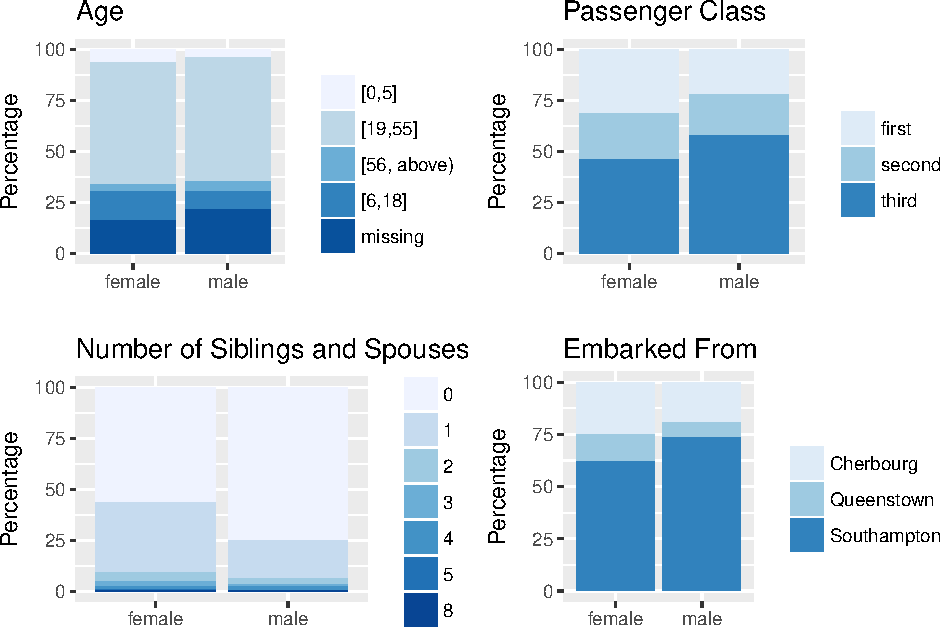
\includegraphics{report_files/figure-latex/unnamed-chunk-8-1.pdf}

It seems that there is not a significant correlation between age and
gender, or gender and embarked from, but there

\hypertarget{conclusion}{%
\chapter{Conclusion}\label{conclusion}}

\hypertarget{findings}{%
\section{Findings}\label{findings}}

\hypertarget{further-study}{%
\section{Further Study}\label{further-study}}

\bibliography{book.bib,packages.bib}

\end{document}
